%As a local optimization strategy, the dynamic pushing primitive does not provide %guaranteed success. In the semi-structured setup of this work, however, it %provides a significant boost to robustness. 

\begin{figure*}
\centering
\begin{tabular}{@{}c@{}c@{}}
%\cline{2-2}
& No corrective actions\\
\multirow{3}{*}{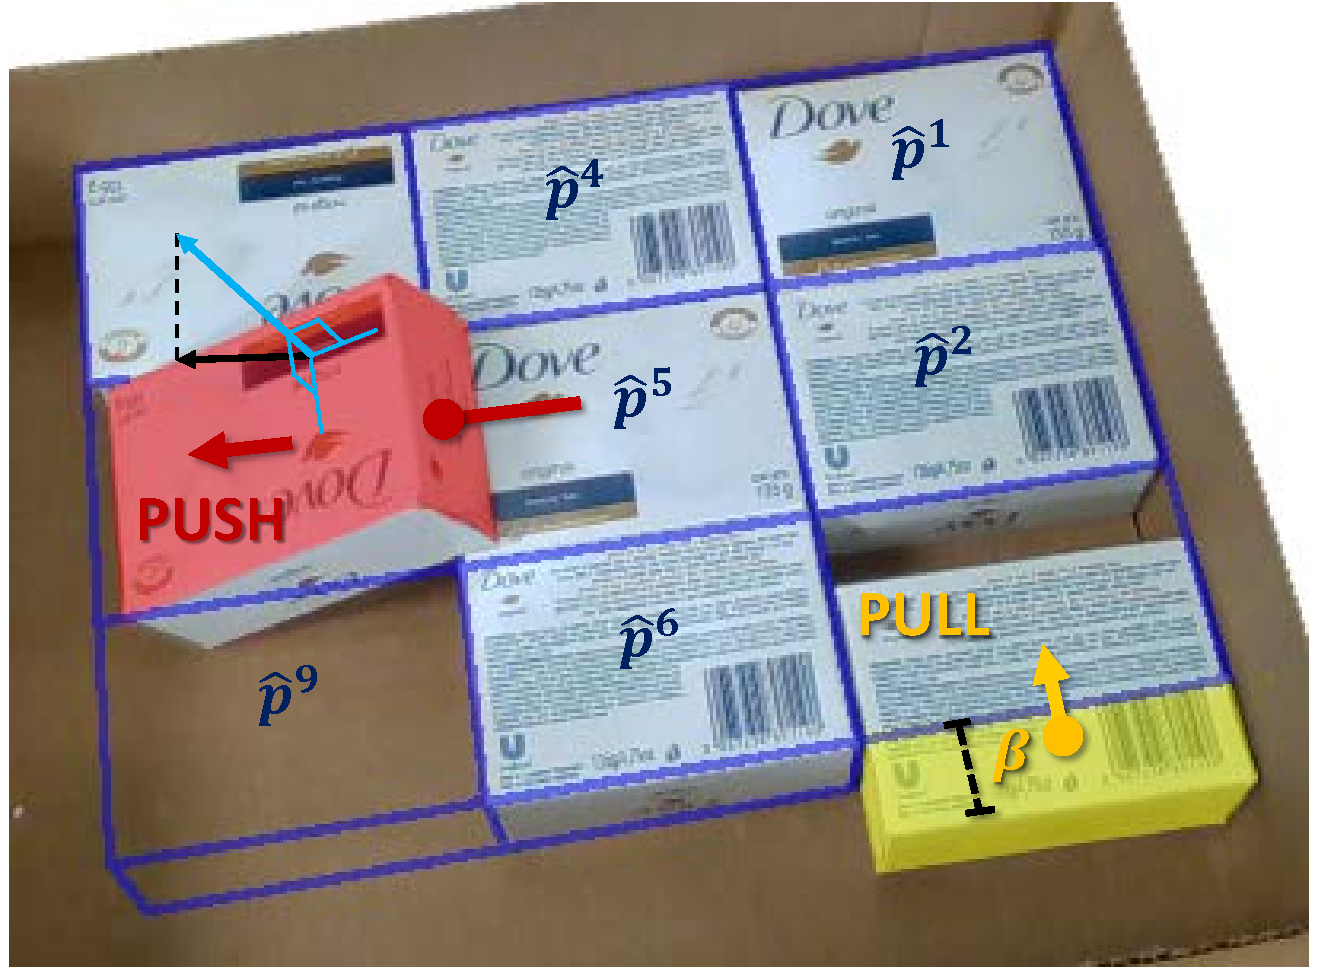
\includegraphics[width=0.24\textwidth]{Figures/finer_fix.pdf}}
& 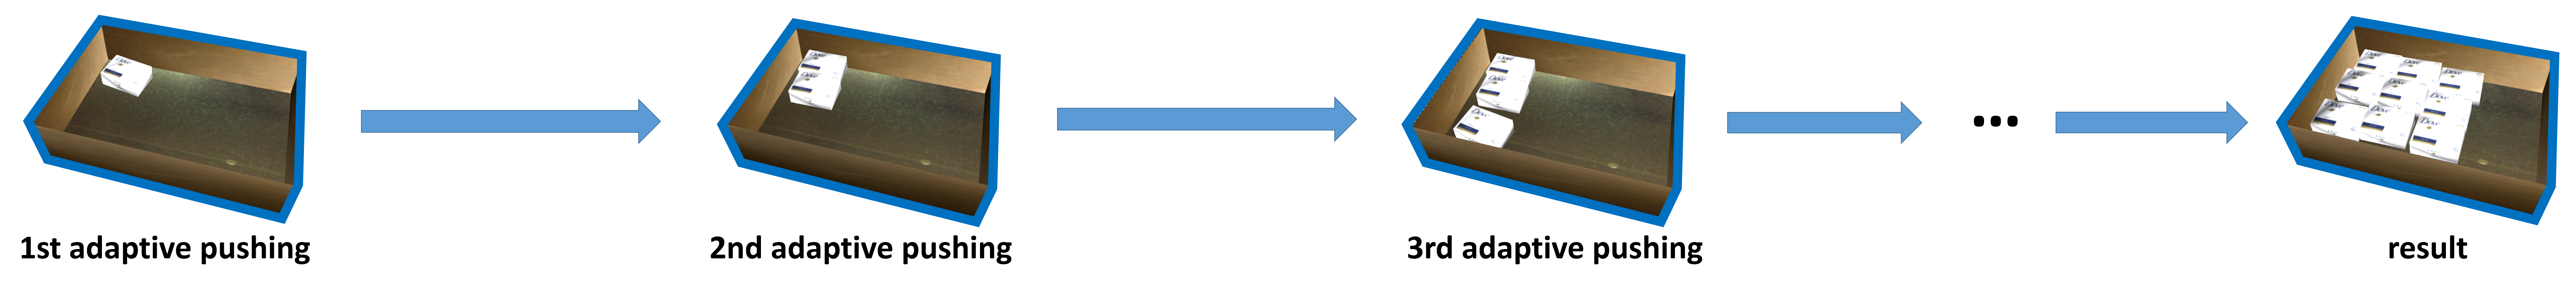
\includegraphics[width=0.75\textwidth,valign=t]{./Figures/res_step_adaptive.png}
\\\cline{2-2}
& Full pipeline\\
& 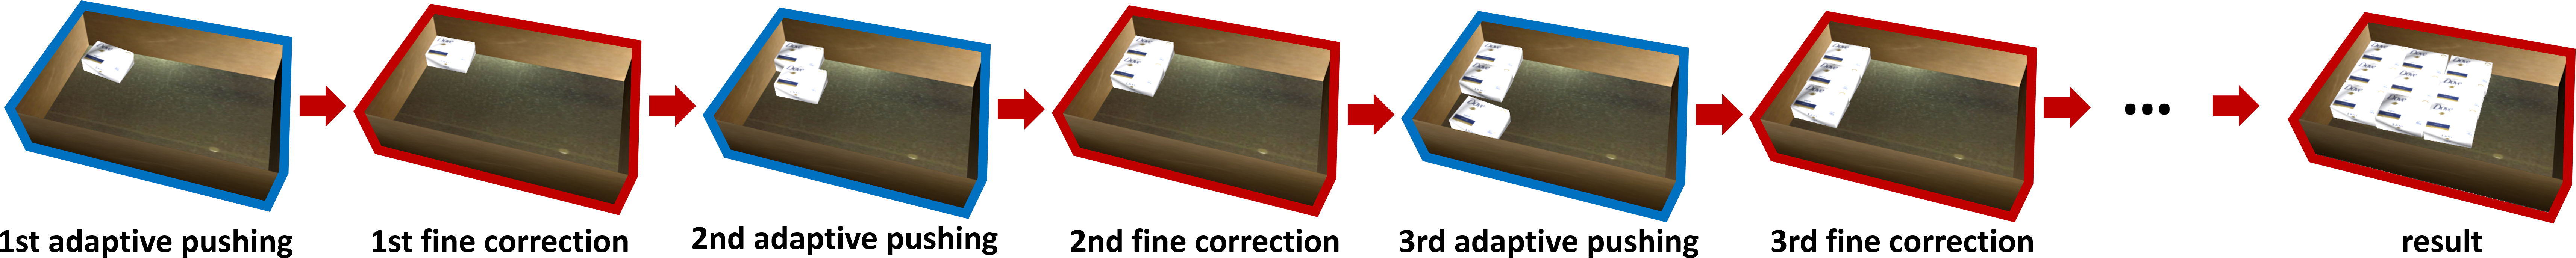
\includegraphics[width=0.75\textwidth]{./Figures/res_step_full.png}
\\%\cline{2-2}
\end{tabular}
\caption{Fine layout adjustment and correction.}
\label{fig:finer_fix}
\end{figure*}

The final primitive deals with the remaining failure cases. Fine corrections are required because objects can be placed in incorrect poses due to unexpected collisions as well as calibration and pose estimation errors.  The proposed corrective manipulation procedure continuously monitors the scene and triggers corrective actions whenever necessary. 

%Even small alignment errors can have a domino effect on the  packing task and make the placement of remaining objects infeasible. 

\begin{comment}
\begin{wrapfigure}{r}{1.5in}
\vspace{-.2in}
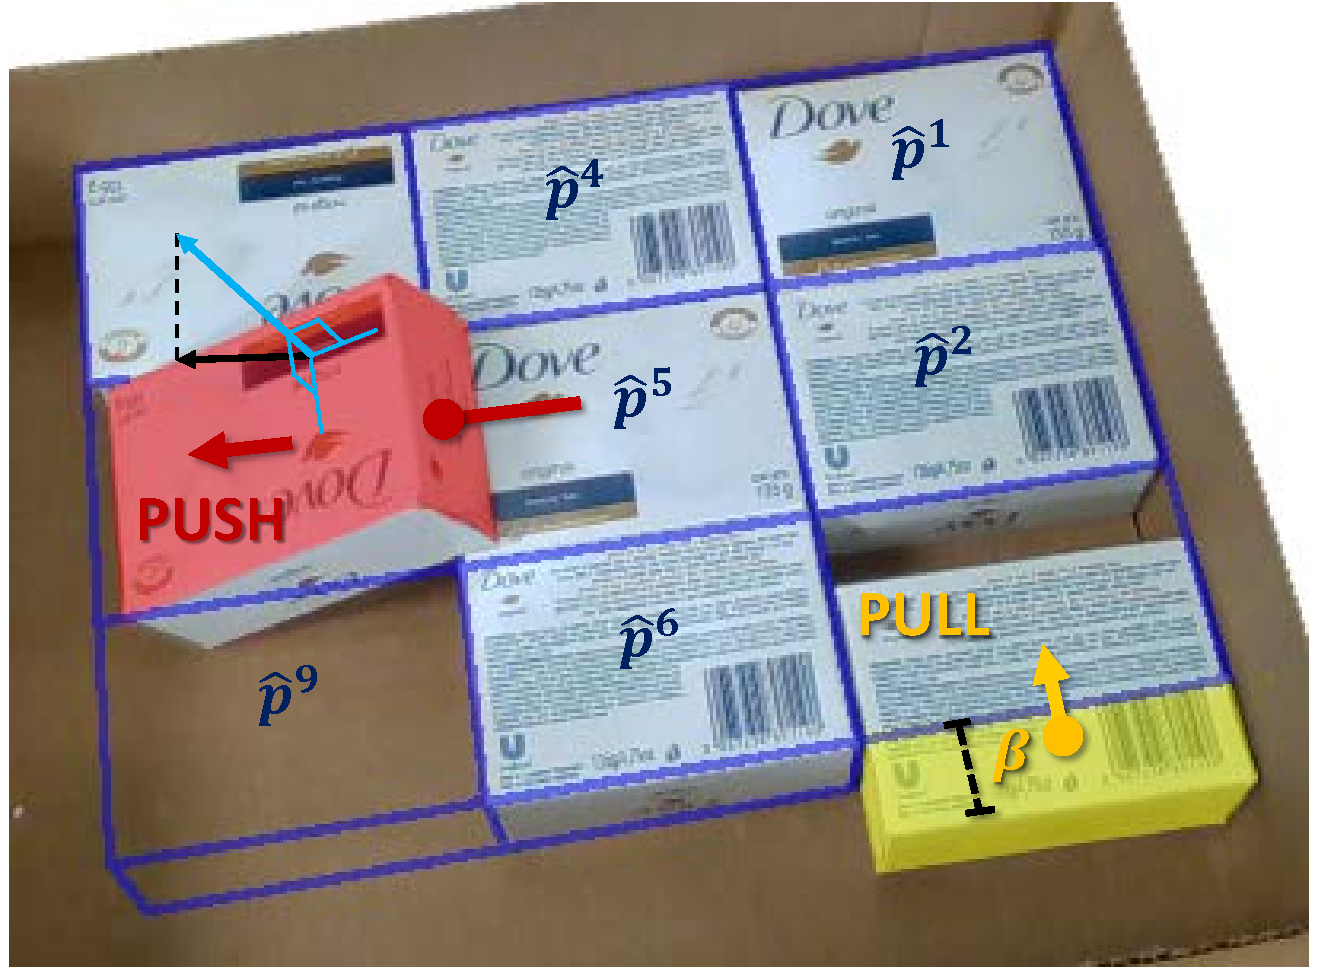
\includegraphics[width=1.49in]{Figures/finer_fix.pdf}
\vspace{-.3in}
\caption{Fine layout adjustment and correction.}
\label{fig:finer_fix}
\vspace{-.15in}
\end{wrapfigure}
\end{comment}

The process first removes the background, the box, the robot's arm and end-effector from the observed point cloud and computes its surface normals.
The observed point cloud is then compared against the desired alignment of the objects in their target poses. As shown in Fig.~\ref{fig:finer_fix}, two types of misalignment errors can occur. The first type occurs when the top surface normal of an object is not perpendicular to the support surface. This error is corrected by pushing the object along a direction and for a distance computed based on its surface normal in a manner that makes it aligned with the support surface. 
The second type of error happens when a peripheral object is not entirely within the desired footprint of the pile. The proposed procedure systematically detects pivot points that are outside the desired footprint of the pile and pulls their objects inside accordingly. The correction is repeated until the point cloud is  aligned with the desired goal poses given a threshold
%$\epsilon$
\changkyu{$\tau$}, or a timeout occurs.

\changkyu{
% [changkyu] uncommented 

Given the alignment pose $\hat{\pose}^i$ which defines the six \textit{facets} $\hat{F}^i = \{\hat{f}_1^i,\dots,\hat{f}_6^i\}$ of the cubic, the pre-processed observation $\mathcal{I}$ is split into disjoint sets $\{X^i\}_{i=0}^n$ where $X^i$ is the point cloud cropped by $\hat{F}^i$ and $X^0$ is the remaining.
Starting with the furthermost point cloud $X^i$ from a pivot point $x_{pivot}$, e.g. the upper right corner of the box, we determine if it agrees with $\atarget$ by measuring the distance between the point cloud $X^i$ and the closest facet $\hat{f}_j^{i'}$ that is not in parallel to the xy-plane as well as the normal difference.
Once a disagreement is detected, an appropriate pushing or pulling action is executed as described in Algorithm \ref{algo:FinerFix}.
For example, the objects leaning against other objects, which accompany a significant normal disagreement, will be pushed away to be slipped, and the objects translated from its desired position will be pulled towards it.
The correction is repeated until all the observation agree with $\atarget$ or timeout.

{\small
\begin{algorithm}
\KwIn{
	$\atarget = \{ \hat{p}^1, \ldots, \hat{p}^n \}$, an error threshold $\tau$, the point cloud segments $\{X[i]\}_{i=0}^{n}$, a corner point $x_{pivot}$
}
\Repeat{Timeout}
{
Sort centers of $X[i]$ based on increasing distance to $x_{pivot}$;\\

	\For{$i\leftarrow 0; i\leq n; i\leftarrow i+1$}
	{
		{\scriptsize\tcp{Check if X[i] is not horizontally placed}}
		\If{ $\{x | normal(x).z < 1 - \epsilon, x \in X[i]\} \neq \emptyset$ }
		{
        Push segment $X[i]$ from a side to translate its center $x_c$  with  $\alpha \times normal(x_c)$, after projecting vector $normal(x_c)$ to the XY plane, and where $\alpha$ is a small constant; \\
			break
		}
		{\scriptsize\tcp{Check if X[i] is horizontally off-set}}
        Let object\_box($\hat{p}^{i'}$) be the closest target to $X[i]$, and let $\beta$ be the {\it Frechet distance} between $X[i]$ and object\_box($\hat{p}^{i'}$).\\
%		\If{ $X[i]$ does not fit with $\hat{p}^i$ }
		{			
			\If{$\beta > \tau$}
			{
				Pull $X[i]$ toward $\hat{p}^{i'}$ with distance $\beta$;\\
				break
			}
		}
	}
	break
}
\caption{Realignment}
\label{algo:FinerFix}
\end{algorithm}
}

}

\begin{comment}
{\small
\begin{algorithm}
\KwIn{
	$\atarget = \{ \hat{p}^1, \ldots, \hat{p}^n \}$, an error threshold $\tau$
}
\Repeat{Timeout}
{
Get {\tt RGB-D} input $\mathcal{I}$;\\
\For{$i := 1; i \leq n; i\leftarrow i+1$}
{
	{\scriptsize\tcc{X[i]: point cloud segment for $o^i$}}
    $X[i] \leftarrow \mathcal{I} \cap \text{object\_box}(\hat{p}^i)$,
	$\mathcal{I} \leftarrow \mathcal{I} \backslash X[i]$
    
}
$X[0] = \mathcal{I}$;\\
$x_{pivot}$ is any corner point in the convex hull of $\mathcal{I}$;\\
Sort centers of $X[i]$ based on increasing distance to $x_{pivot}$;\\

	\For{$i\leftarrow 0; i\leq n; i\leftarrow i+1$}
	{
		{\scriptsize\tcc{Check if X[i] is not horizontally placed}}
		\If{ $\{x | normal(x).z < 1 - \epsilon, x \in X[i]\} \neq \emptyset$ }
		{
        Push segment $X[i]$ from a side to translate its center $x_c$  with  $\alpha \times normal(x_c)$, after projecting vector $normal(x_c)$ to the XY plane, and where $\alpha$ is a small constant; \\
			break
		}
		{\scriptsize\tcc{Check if X[i] is horizontally off-set}}
        Let object\_box($\hat{p}^{i'}$) be the closest target to $X[i]$, and let $\beta$ be the {\it Frechet distance} between $X[i]$ and object\_box($\hat{p}^{i'}$).\\
%		\If{ $X[i]$ does not fit with $\hat{p}^i$ }
		{			
			\If{$\beta > \tau$}
			{
				Pull $X[i]$ toward $\hat{p}^{i'}$ with distance $\beta$;\\
				break
			}
		}
	}
	break
}
\caption{Realignment}
\label{algo:FinerFix}
\end{algorithm}
}
\end{comment}